\subsection{高并发及事务管理}
\subsubsection{高并发}
支持百万级别的高并发大数据流量已成为现代数据库系统的设计性能标准。在第二部分的最后,我们通过异步使用连接池,利用了数据库的高并发支持,在约两分钟的时间段内,数据库持续承受住了20个连接的写入操作。关于高并发的一个常见问题是\emph{死锁}。“加锁(Locking)是数据库在并发访问时保证数据一致性和完整性的主要机制。任何事务都需要获得相应对象上的锁才能访问数据,读取数据的事务通常只需要获得读锁(共享锁),修改数据的事务需要获得写锁(排他锁)。当两个事务互相之间需要等待对方释放获得的资源时,如果系统不进行干预则会一直等待下去,也就是进入了死锁(deadlock)状态。”\textsuperscript{\cite{dong-2021}}\\~\\
\centerline{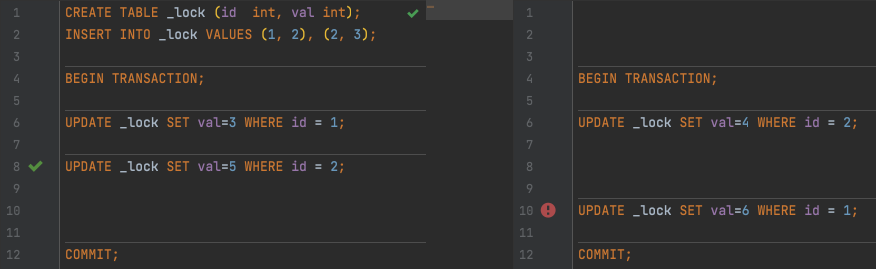
\includegraphics[width=0.8\textwidth]{sp/lkdemo}}
\par 上图尝试在不同事务中以不同的顺序修改数据,首先在左事务中修改id为1的数据,此部分被加锁、右事务修改id为2的数据,同样加锁;第二步让左事务修改id为2的数据,但此时DBMS为避免脏写,已经为其加上写锁,因此左事务的进程需要等待右事务结束以释放写锁;在左事务的等待状态中,右事务修改被左事务添加写锁的数据,此时右事务也进入等待状态;注意到左事务一直在等待右事务结束以释放写锁,而右事务也在等待左事务释放写锁以执行命令并结束,两个事务进入了互相等待对方资源的状态,这种等待是无限的。但现在大部分数据库都能在等待一段时间后检查出死锁,并做出\emph{终止一个事务并让另一个事务成功执行}的调度(如下图)。但是一个事务长期等待另一个事务释放资源并不会引起DBMS的介入。\\~\\
\centerline{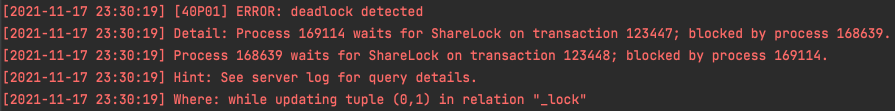
\includegraphics[width=0.85\textwidth]{sp/dlock}}


\subsubsection{事务管理}
事务管理主要为RDBMS提供了\emph{原子性 (Atomicity)、一致性 (Consistency)、隔离性 (Isolation)和持久性 (Durability)}这四大特性\textsuperscript{\cite{silberschatz-2010}}。
\paragraph{原子性} 指一个事务块中的所有事件或全部成功执行,或全不执行,即在中间任何一个事件失败时需要回滚指事务开始时的状态。在事务块中遇到第一个错误后,Postgres会忽略后面的命令,直至执行一次\textbf{ROLLBACK}回滚至事务开始时的状态,或执行\textbf{COMMIT}并由DBMS丢弃此事务块的所有影响。此外,即使所有操作成功执行,用户也可使用ROLLBACK取消所做修改。
\begin{figure*}[!h]
	\centering
	\begin{subfigure}[b]{0.3\textwidth}
		\centerline{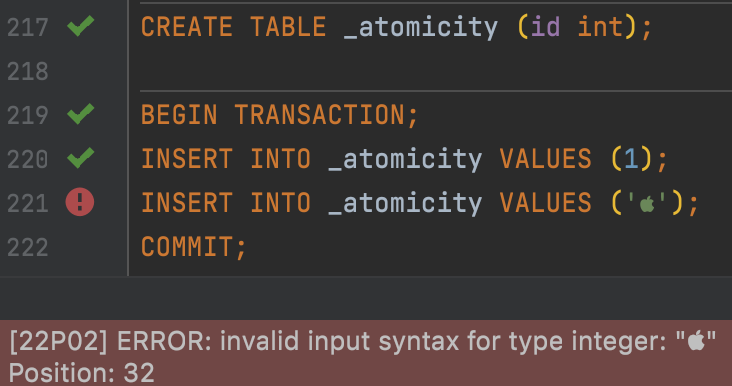
\includegraphics[height=2.7cm]{./sp/trs1}}
		\caption{事务块中出现错误}
	\end{subfigure}
	\\
	\begin{subfigure}[b]{0.3\textwidth}
		\centerline{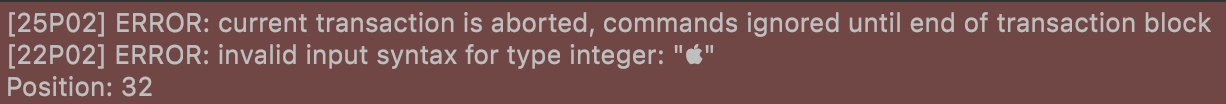
\includegraphics[height=0.7cm]{./sp/trs2}}
		\caption{提示当前事务块所有会被取消}
	\end{subfigure}
	\\
	\begin{subfigure}[b]{0.9\textwidth}
		\centerline{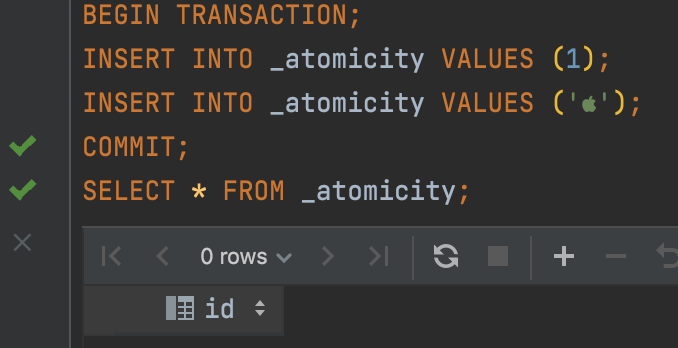
\includegraphics[height=2.7cm]{./sp/trs3}}
		\caption{执行COMMIT,此时DBMS取消了事务中的操作,查询结果所示与事务开始前状态一致}
	\end{subfigure}
	\\
	\begin{subfigure}[b]{0.9\textwidth}
		\centerline{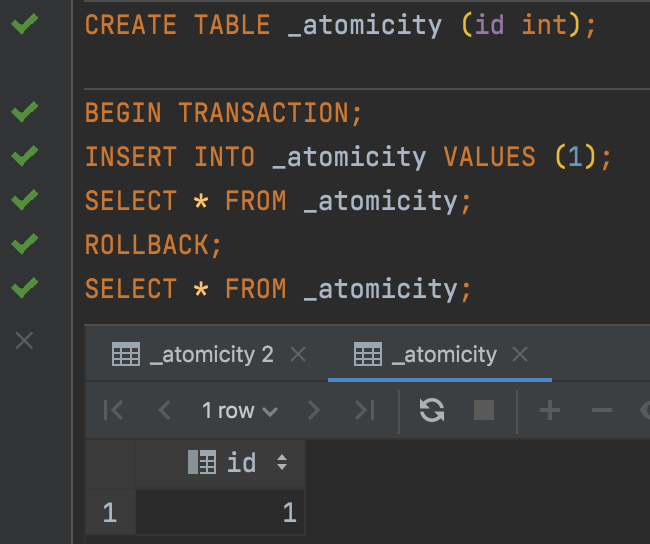
\includegraphics[height=2.75cm]{./sp/trs4}\qquad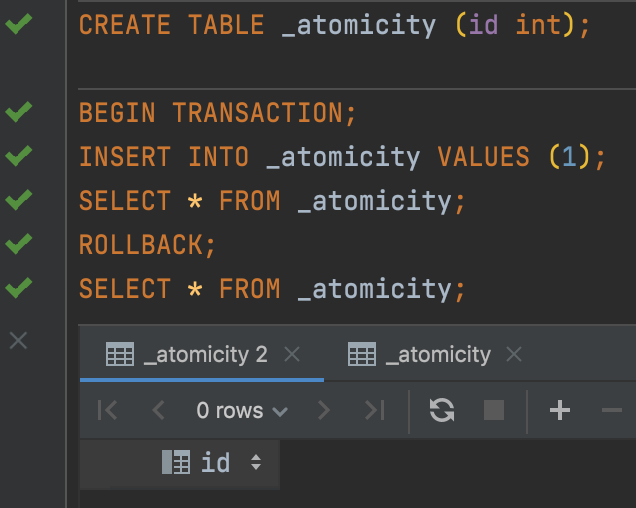
\includegraphics[height=2.75cm]{./sp/trs5}}
		\caption{左图示成功插入一条数据,执行回滚后再次查询,结果与事务开始前一致}
	\end{subfigure}
\end{figure*}

\paragraph{一致性} 报告第二部分插入数据即利用了此特性。出于各种原因,人们可能不关心某件事中间过程的高度一致,而仅要求事件前后均满足各种限制即可。“在事务开始之前和事务结束以后,数据库的完整性没有被破坏。这表示写入的资料必须完全符合所有的预设约束、触发器、级联回滚等。”\textsuperscript{\cite{acid-wiki}}
\begin{figure*}[!h]
	\centering
	\begin{subfigure}[b]{0.9\textwidth}
		\centerline{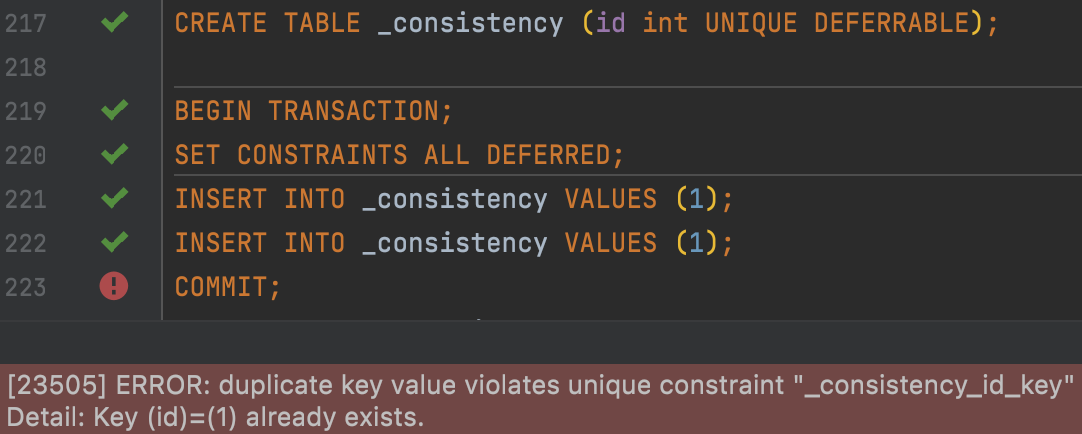
\includegraphics[height=2.7cm]{./sp/trs6}\qquad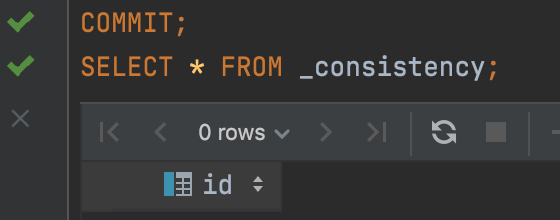
\includegraphics[height=2.7cm]{./sp/trs7}}
		\caption{延迟检查使事务块中可违反一些约束,而在COMMIT前会检查一致性并报错}
	\end{subfigure}
\end{figure*}

\paragraph{隔离性} “数据库允许多个并发事务同时对其数据进行读写和修改的能力,隔离性可以防止多个事务并发执行时由于交叉执行而导致数据的不一致。事务隔离分为不同级别,包括未提交读(read uncommitted)、提交读(read committed)、可重复读(repeatable read)和串行化(serializable)。”\textsuperscript{\cite{acid-wiki}}
\par 以下测试均在DataGrip中使用console建立一个连接,并在CLI中使用另一角色登录并修改数据,以此模拟并发读写。
\subparagraph{读已提交} 下面的实验展示在读已提交的隔离级别中,一个查询只能看到查询开始前已提交的数据(查询开始瞬间的数据库快照),无法看到未提交或查询期间由其他事物提交的数据,但查询可看见自身事务中之前执行的更新。读已提交不会导致\emph{脏读}(即一个事务读取了另一个未提交的事务写入的数据),同时也是PostgreSQL的默认隔离级别。但读已提交也可能造成不可重复读,即同一事务中两个相邻查询返回的结果可能不同,这是因为在两次查询开始的间隔中可能有其他事务被提交。
\begin{lstlisting}
conn1=# CREATE TABLE _isolation (id  int, val int);
conn1=# SELECT * FROM _isolation;
 id | val 
----+-----
(0 rows)

conn1=# BEGIN TRANSACTION;
conn1=# SET TRANSACTION ISOLATION LEVEL READ COMMITTED;
conn2=# BEGIN TRANSACTION;
conn2=# INSERT INTO _isolation VALUES (2, 1);
conn1=# SELECT * FROM _isolation;
 id | val 
----+-----
(0 rows)

conn2=# COMMIT;
conn1=# SELECT * FROM _isolation;
 id | val 
----+-----
  2 |   1
(1 row)
\end{lstlisting}
\vspace{-2em}

\subparagraph{可重复读} 与读已提交的一个非常相似的隔离级别是可重复读,其只允许读取已提交数据,且一个事务两次读取一个数据项期间,不允许其他事务更新该数据,即一个可重复读事务中的查询可以看见在事务中第一个非事务控制语句开始时的一个快照。但其与读已提交一样,依然可能出现幻读。
\begin{lstlisting}
conn1=# CREATE TABLE _isolation (id  int, val int);
conn1=# BEGIN TRANSACTION;
conn1=# SET TRANSACTION ISOLATION LEVEL REPEATABLE READ;
conn2=# BEGIN TRANSACTION;
conn2=# INSERT INTO _isolation VALUES (2, 1);
conn2=# COMMIT;
conn1=# SELECT * FROM _isolation;
 id | val 
----+-----
(0 rows)

conn1=# COMMIT;
conn1=# SELECT * FROM _isolation;
 id | val 
----+-----
  2 |   1
(1 row)
\end{lstlisting}
\vspace{-2em}

\subparagraph{可串行化} 是四种隔离级别中唯一避免了\emph{幻读}\footnote{一个事务开始后,需要根据数据库中现有的数据做一些更新,于是重新执行一个查询,返回符合查询条件的行,这时发现这些行因为其它最近提交的事务而发生了改变,导致现有事务如果再进行下去可能发发生逻辑上的错误。}的级别,也即是最高的事务隔离级别,在该级别下,事务串行化顺序执行,可以避免脏读、不可重复读与幻读\footnote{不可重复读对应的是修改,即UPDATE操作;而幻读问题对应的是INSERT操作。}。但是这种事务隔离级别效率低下,比较耗数据库性能,不常用。

\subparagraph{读未提交} 允许读取未提交的数据,是SQL允许的最低一致性级别。可能导致脏读、不可重复读以及幻读(但对于PostgreSQL,此级别的行为与读已提交相同,因为DBMS内部实际上只实现了另外三种隔离级别)。另外,以上四种隔离级别均不允许脏写。


\paragraph{持久性} 事务块成功结束后,对数据的修改就是永久的,即便系统故障也不应丢失。如下图所示,将postgres.service强制突然kill掉,模拟系统突然故障,此后重新启动服务,检查数据库存储条目与kill前一致(kill前已结束事务)。\\~\\
\centerline{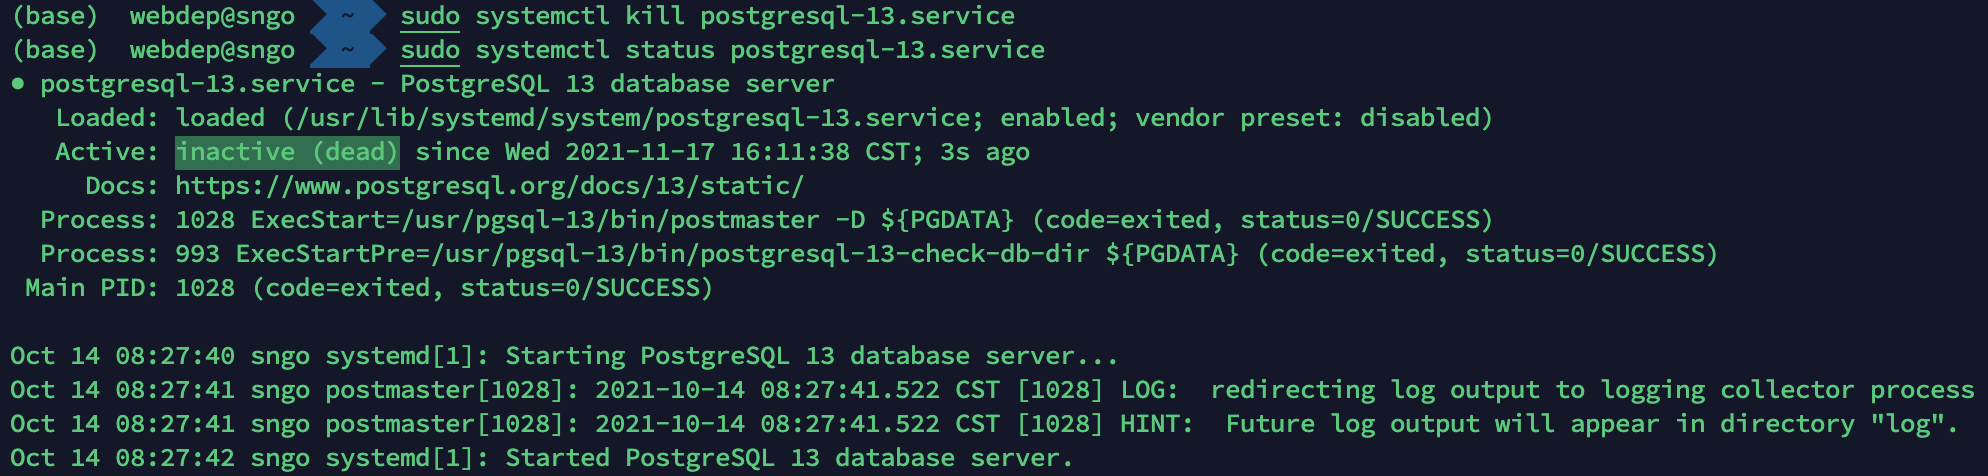
\includegraphics[width=0.7\textwidth]{sp/kill}}